\documentclass[12pt, a4paper]{article}
\usepackage[UTF8]{ctex}
\usepackage{amsmath}
\usepackage{amssymb}
\usepackage{amsthm}
\usepackage{geometry}
\usepackage{enumitem}
\usepackage{indentfirst}
\usepackage{caption}
\usepackage{fancyhdr}
\usepackage{booktabs}
\usepackage{titlesec}
\usepackage{draftwatermark}
\usepackage{graphicx} % 导入图像的宏包、单图





% 页面布局设置
\geometry{top=2.54cm, bottom=2.54cm, left=3.18cm, right=3.18cm}

% 行距设置
\linespread{1.5}

%设置水印
\SetWatermarkText{B站：布加拉提}
\SetWatermarkScale{0.4}
% 段落设置
\setlength{\parindent}{2em}
\setlength{\parskip}{0.5em}

% 节标题格式设置
\titleformat{\section}{\normalfont\Large\bfseries}{第\chinese{section}章、}{1em}{}
\titlespacing{\section}{0pt}{2.5ex plus 1ex minus .2ex}{1.3ex plus .2ex}

% 定理环境设置
\newtheoremstyle{solution}
{}
{}
{}
{}
{\bfseries}
{、}
{1em}
{}
\theoremstyle{solution}
\newtheorem{sol}{解}

% 页眉页脚设置
\pagestyle{fancy}
\fancyhf{}
\fancyhead[C]{b站布加拉提整理（回忆版）b站甘茶w独家讲解}
\fancyfoot[C]{\thepage}

\rfoot{整理人：八方\\资源提供：考研乔瑟夫}
\lhead{
\includegraphics[width=0.06\linewidth]{p1.png}}
\rhead{
\includegraphics[width=0.06\linewidth]{p2.png}}
\renewcommand{\headrulewidth}{0.4pt}
\renewcommand{\footrulewidth}{0.4pt}

\begin{document}

\begin{center}
\Large\textbf{2004哈工大硕士考试试题：805物理光学}
\end{center}




\section*{一、选择与填空（共8题，32分）}
\begin{enumerate}
    \item 当一束自然光以布儒斯特角入射到两种介质分界面上时，就偏振态来说反射光为\_\_\_\_\_，其振动方向 \_\_\_\_\_入射面，透射光为\_\_\_\_\_.
    \item 若某一激光的频宽\(\Delta \nu=5.4×10^4HZ\)则这一激光的波列长度是\_\_\_\_\_.\\$(A)5.55×10^3m \quad (B)1.8×10^3m \quad (C)3.5×10^4m \quad (D)5.55×10^4m$
    \item 假设某一介质对空气的临界角是45度，则光从空气射向此介质的布儒斯特角是\_\_\_\_\_.
    \item（重复）在真空中波长为\(\lambda\)的单色光,在折射率为n的透明介质中从A沿路径传播到B，若若A,B两点的相位差为3\(\pi\) ,则此路径AB地光程差为\_\_\_\_\_.\\(A)1.5\(\lambda\) \qquad(B)1.5\(n\lambda\) \qquad(C)3\(\lambda\) \qquad(D)1.5\(\lambda/n\)
    \item 波长为\(\lambda\)的单色平行光垂直入射到一狭缝上，若第一级暗纹的位置对应的衍射角为$\theta=±\pi/6$,则缝宽的大小为\_\_\_\_\_.\\(A)\(\lambda/2\)\qquad(B)\(\lambda\)\qquad(C)\(2\lambda\)\qquad(D)\(4\lambda\)
    \item （重复）波长\(\lambda=550nm\) 的单⾊光垂直⼊射到光栅常数\(d=2×1 0^{-4}cm\)的平面衍射光栅上，能观察 到的光谱线的最⼤级次为:\_\_\_\_ .\\（ A ） 2  \qquad (B)  3\qquad  （ C ）4 \qquad （ D ） 5
    \item （重复）⼀光强为 \(I_0\) 的线偏振光先后通过两个偏振⽚\(p_1\)和\(p_2\) ，\(p_1\) 和\(p_2\) 的偏振⽅向与原⼊射光的光矢量振动⽅向的夹角分别是\(\alpha\) 和 \(90°\)，则通过两偏振⽚后的光强是:\_\_\_\_ .\\(A) 1/2\(I_0 cos^2\alpha\)  \quad(B) 0  \quad(C) 1/4\(I_0 sin^2 2\alpha\)  \quad(D) 1/4\(I_0sin^2a\) \quad (E) \(I_0cos^4 \alpha\)
    \item 若正入射的线偏振光振动方向与半波片的快，慢轴成45°角。半波片的厚度为d。在半波片中距离入射表面为\(d/2\)处两偏振光叠加后的偏振态为:\_\_\_\_ .\\(A)线偏振光\quad (B)园偏振光\quad (C)椭圆偏振光\quad (D)部分偏振光
\end{enumerate}
\section*{二、简述题（共7题，56分）}
\begin{enumerate}
    \item 在一般情况下，单色平面波在各向同性介质中和在晶体中传播有何区别，以单轴晶体为例画图说明。
    \item 画出反射光和入射光中s和p分量的相位关系\(\varphi_s\)和\(\varphi_p\)，$(n_1>n_2)$。并说明线偏振光以大于临界角入射时，反射光的偏振态。
    \item 影响干涉条纹对比度的主要因素有哪些？以杨氏干涉为例说明空间相干性的物理含义。
    \item 平行平板产生的等倾干涉与牛顿环产生的等厚干涉有何异同？如何区分？
    \item 一平行单色光垂直入射到光栅上，在满足$dsin\theta=3\lambda$,经光栅相邻两缝沿\(\theta\) 方向衍射的两束光的光程差是多少？经第1缝和第n缝衍射的两束光的光程差又是多少？这时通过任意两缝的光是否可以相干加强？
    \item （重复）什么是瑞利判据？以望远系统为例说明它对实际光学系统有何意义？
    \item 闪耀光栅与普通光栅相比有什么特点？在原理上如何实现对对某波长光的闪耀？
\end{enumerate}
\section*{三、计算与分析（共3题，32分）}
\begin{enumerate}
    \item 单色光源S照射平行平板G经反射后，通过透镜L在其焦平面E上产生等倾干涉条纹（如图所示）。光源不直接照射透镜，光波长$\lambda=0.6\mu m$,板厚$d=1.6mm$，折射率$n=1.5$,透镜焦距$f=40mm$。若屏E上的干涉中心是暗的。那么屏上所看到的第5个暗环半径是多少？为了在给定的参数下看到干涉环，照在板上的谱线最大允许宽度$\Delta\lambda$又是多少？
    \centerline{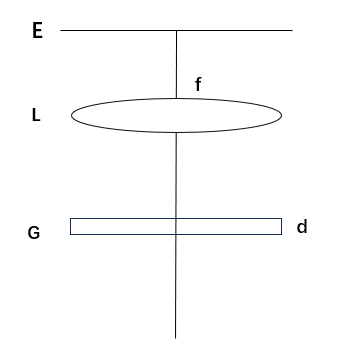
\includegraphics[width=0.3\linewidth]{04.png}}
    \item 一光栅宽为5cm，每毫米内有400条刻线，当波长为$\lambda=0.5\mu m$的平行光垂直入射时，第4级衍射光谱处在单缝衍射的第一极小位置，试求：
    \begin{enumerate}
        \item 每个缝(透光部分)的宽度。
        \item 第二级衍射光谱的半角宽度。
        \item 第二级可分辨的最小波长。
        \item 若入射光改为与光栅平面法线成30度角方向斜入射时，光栅能分辨的最小波长差又为多少？
    \end{enumerate}
    \item 通过偏振片观察部分偏振光时，当偏振片绕入射光方向转到某位置上，投射光强为极大，然后再将偏振片旋转30度发现投射光强为极大值的4/5，试求该入射部分偏振光的偏振度P及该光内自然光与线偏振光强之比。
\end{enumerate}
\section*{四、综合题（30分）}
\begin{enumerate}
    \item 请简述迈克尔逊干涉仪的工作原理，说明它可能有说明用途，根据你的理解，讨论其时间相干性，当光源分别为点光源和扩展光源时，讨论干涉条纹定义域。

\end{enumerate}
\end{document}